\documentclass[11pt]{beamer}
\usepackage{listings} % Include the listings-package
\usepackage[T1]{fontenc}
\usepackage[utf8]{inputenc}
\usepackage[english]{babel}
\usepackage{amsmath}
\usepackage{amssymb, amsfonts, latexsym, cancel}
\usepackage{float}
\usepackage{graphicx}
\usepackage{epstopdf}
\usepackage{subfigure}
\usepackage{hyperref}
%\usepackage{authblk}
\usepackage{blindtext}
\usepackage{booktabs} % Allows the use of \toprule, 
\usepackage{filecontents}
\usepackage{courier} %% Sets font for listing as Courier.
\usepackage{listings}
%\usepackage{listings, xcolor}
\lstset{
tabsize = 2, %% set tab space width
showstringspaces = false, %% prevent space marking in strings, string is defined as the text that is generally printed directly to the console
numbers = left, %% display line numbers on the left
commentstyle = \color{green}, %% set comment color
keywordstyle = \color{blue}, %% set keyword color
stringstyle = \color{red}, %% set string color
rulecolor = \color{black}, %% set frame color to avoid being affected by text color
basicstyle = \small \ttfamily , %% set listing font and size
breaklines = true, %% enable line breaking
numberstyle = \tiny,
}
\usepackage{caption}
\DeclareCaptionFont{white}{\color{white}}
\DeclareCaptionFormat{listing}{\colorbox{gray}{\parbox{\textwidth}{#1#2#3}}}
\captionsetup[lstlisting]{format=listing,labelfont=white,textfont=white}
\definecolor{urlColor}{rgb}{0.06, 0.3, 0.57}
\definecolor{linkColor}{rgb}{0.57, 0.0, 0.04}
\definecolor{fileColor}{rgb}{0.0, 0.26, 0.26}
\hypersetup{
    colorlinks=true,
    linkcolor=linkColor,
    filecolor=fileColor,      
    urlcolor=urlColor,
}
\urlstyle{same}
\setbeamercovered{transparent}
%\usetheme{Boadilla}
\usetheme{CambridgeUS}
%\usetheme{Berkeley}
%\usetheme{Warsaw}
%\usetheme{Madrid}

\title[Introducción]{\bf\Huge Instrucción en uso de videojuegos}
\subtitle{Interacción Humano Computador}

\author[rescobedoq]
{
	Jeampier Anderson Moran Fuño \inst{1}\\
	Marcelo Andre Guevara Guitierrez\inst{1}\\
	Rony Tito Ventura Ramos\inst{1}\\
	Rudy Roberto Tito Durand\inst{1}
}
\institute[UNSA]
{
\inst{1}% 
System Engineering School\\
System Engineering and Informatic Department\\
Production and Services Faculty\\
San Agustin National University of Arequipa
}

\date[2020-15-09]{\scriptsize{2020-15-09}}
%\logo{\includegraphics[width=3.0cm]{img/logo_unsa.jpg}}
\titlegraphic{\includegraphics[width=1.0cm]{img/logo_unsa.jpg}}

\begin{document}

\begin{frame}
\titlepage
\end{frame}

\begin{frame}
\frametitle{Content}
\tableofcontents
\end{frame}

\section{Aqui Pondremos la primera Diapo}
\begin{frame}
\frametitle{Introducción}
Los videojuegos son una de las principales formas de entretenimiento entre niños y jóvenes y su industria se ha desarrollado a la par del desarrollo de las tecnologías de la información. El crecimiento de la industria de los videojuegos en las últimas décadas ha sido tal que ya ha superado la facturación del cine y la música juntos. Además de su importancia económica, algunos videojuegos han sido denominados como obras de arte y muchos consideran que el desarrollo y diseño de videojuegos debería ser considerado el octavo arte, ya que se necesita mucha imaginación e inspiración para crear un universo que se puede usar para desarrollar un videojuego .

La innovación y el desarrollo tecnológico están estrechamente relacionados con el desarrollo de los videojuegos y cada vez nos sorprende más la estética y la jugabilidad de los últimos juegos lanzados.

\end{frame}

\section{Elegir el estilo del juego}
\begin{frame}
\frametitle{Elección de tu estilo propio en un videojuego}
Al momento de crear un videojuego el primer paso es pensar el estilo ya que será nuestra base para empezar con todo el desarrollo no solo de las partes tecnicas sino tambien las emociones que queremos transmitirle con nuestro juego.
\begin{center}
 \includegraphics[scale=0.2,keepaspectratio=true]{img/estilos de juego.jpg}
 % estilos de juego.jpg: 455x463 px, 96dpi, 12.04x12.25 cm, bb=0 0 341 347
\end{center}
\end{frame}

\section{Importancia del color}
\begin{frame}
\frametitle{La importancia del color en los videojuegos}
\begin{itemize}
\item Los diseñadores usan colores para definir estados de ánimo y para transmitir sensaciones a los jugadores. SI se usan junto con la iluminación sirven para crear atmosferas de juego en el diseño de escenarios, y para definir la disposición de un personaje.

\item Muchos desarrolladores escogen un color que va a identificar al juego y lo desarrolan con el fin de que este color conecte con el jugador mostrándole los principales conceptos del juego.
\end{itemize}
\end{frame}

\section{Colores Frios y Calientes}
\begin{frame}
\frametitle{Colores Frios y Calientes}
\begin{itemize}
\item Los colores complementarios se encuentran opuestos unos de otros en la rueda de colores y al colocarlos juntos se crea un efecto dinámico y se potencia su brillantez. Los colores análogos se sitúan uno al lado del otro y al juntarlos crean un efecto relajante y armonioso. 
\item El tono (es la variación cualitativa del color), la saturación (es la cantidad de pigmento y pureza del color) y la luminosidad (es el nivel de blancos y negros en el color). 
\end{itemize}
\end{frame}

\section{Colores complementarios}
\begin{frame}

\begin{center}
 \includegraphics[scale=0.7,keepaspectratio=true]{img/colorgama.png}
 % colorgama.png: 455x463 px, 96dpi, 12.04x12.25 cm, bb=0 0 341 347
\end{center}

\end{frame}
\section{Diseño de personajes}
\subsection{Borradores y bocetos}
\begin{frame}
\frametitle{Diseño de personajes}
\framesubtitle{Borradores y bocetos}
\begin{itemize}
\item Un boceto es una copia fisica de una idea, los diseñadores normalmente  utilizan esas copias para ir creando hilos, conceptos para que el mundo de nuestro videojuego tome forma.
\end{itemize}
\begin{center}
 \includegraphics[scale=0.05,keepaspectratio=true]{img/BOCETOS_oso.png}
\end{center}
\end{frame}

\subsection{Conceptualización}
\begin{frame}
\frametitle{Diseño de personajes}
\begin{itemize}
\item Estudiar los proporciones corporales de nuestro personaje.
\item Si es animal se tendra que estudiar las caracteristicas corporales del animal esocogido.
\item Si es un vegetal se tendra que estudiar sus caracteristicas al igual que en el anterior caso.
\end{itemize}
\framesubtitle{Conceptualización}
\begin{center}
 \includegraphics[scale=0.6,keepaspectratio=true]{img/conceptualizacion.png}
\end{center}
\end{frame}

\subsection{Movimiento}
\begin{frame}
\frametitle{Diseño de personajes}
\begin{itemize}
\item Los movimento de nuestros personajes debe ser de acuerdo a su conceptualización.
\item Recomendaciones
	\begin{itemize}
	\item 	La velocidad del juego no debe ser muy alta ni muy baja.
	\item 	Se debe intentar transmitir un mensaje en cada movimiento.
	
	\end{itemize}
\end{itemize}
\framesubtitle{Movimiento}
\begin{center}
 \includegraphics[scale=0.15,keepaspectratio=true]{img/lapiz.png}
\end{center}
\end{frame}

\subsection{Jugabilidad}
\begin{frame}

\frametitle{Diseño de personajes}
\framesubtitle{Jugabilidad}
	\begin{itemize}
	\item Es importante que la interfaz que el usuario tendra con nuestro personaje sea intuitiva.
	\item Es importante agregar una breve descripcion de las acciones a realizar en cada escenario del juego.
	\item Sensacion de progreso.
	\item Si el juego genera adiccion, podria tomarse como indicio que tiene una exelente trama y jugabilidad, si se dirige esta adiccion se podria obtener resultados exepcionales.
	\end{itemize}
\end{frame}


\section{Diseño de Escenario}
\subsection{Historia del Escenario}
\begin{frame}

\frametitle{Diseño de Escenario}
\framesubtitle{Historia del Escenario}
	\begin{itemize}
	\item Un buen diseño aumenta la jugabilidad del videojuego.
	\item El escenario tiene que ser el gran protagonista de la historia.
	\item Es importante el nivel de detalles.
	\end{itemize}
\end{frame}

\subsection{Dinamicas Compositivas}
\begin{frame}

\frametitle{Diseño de Escenario}
\framesubtitle{Dinamicas Compositivas}
\begin{center}


 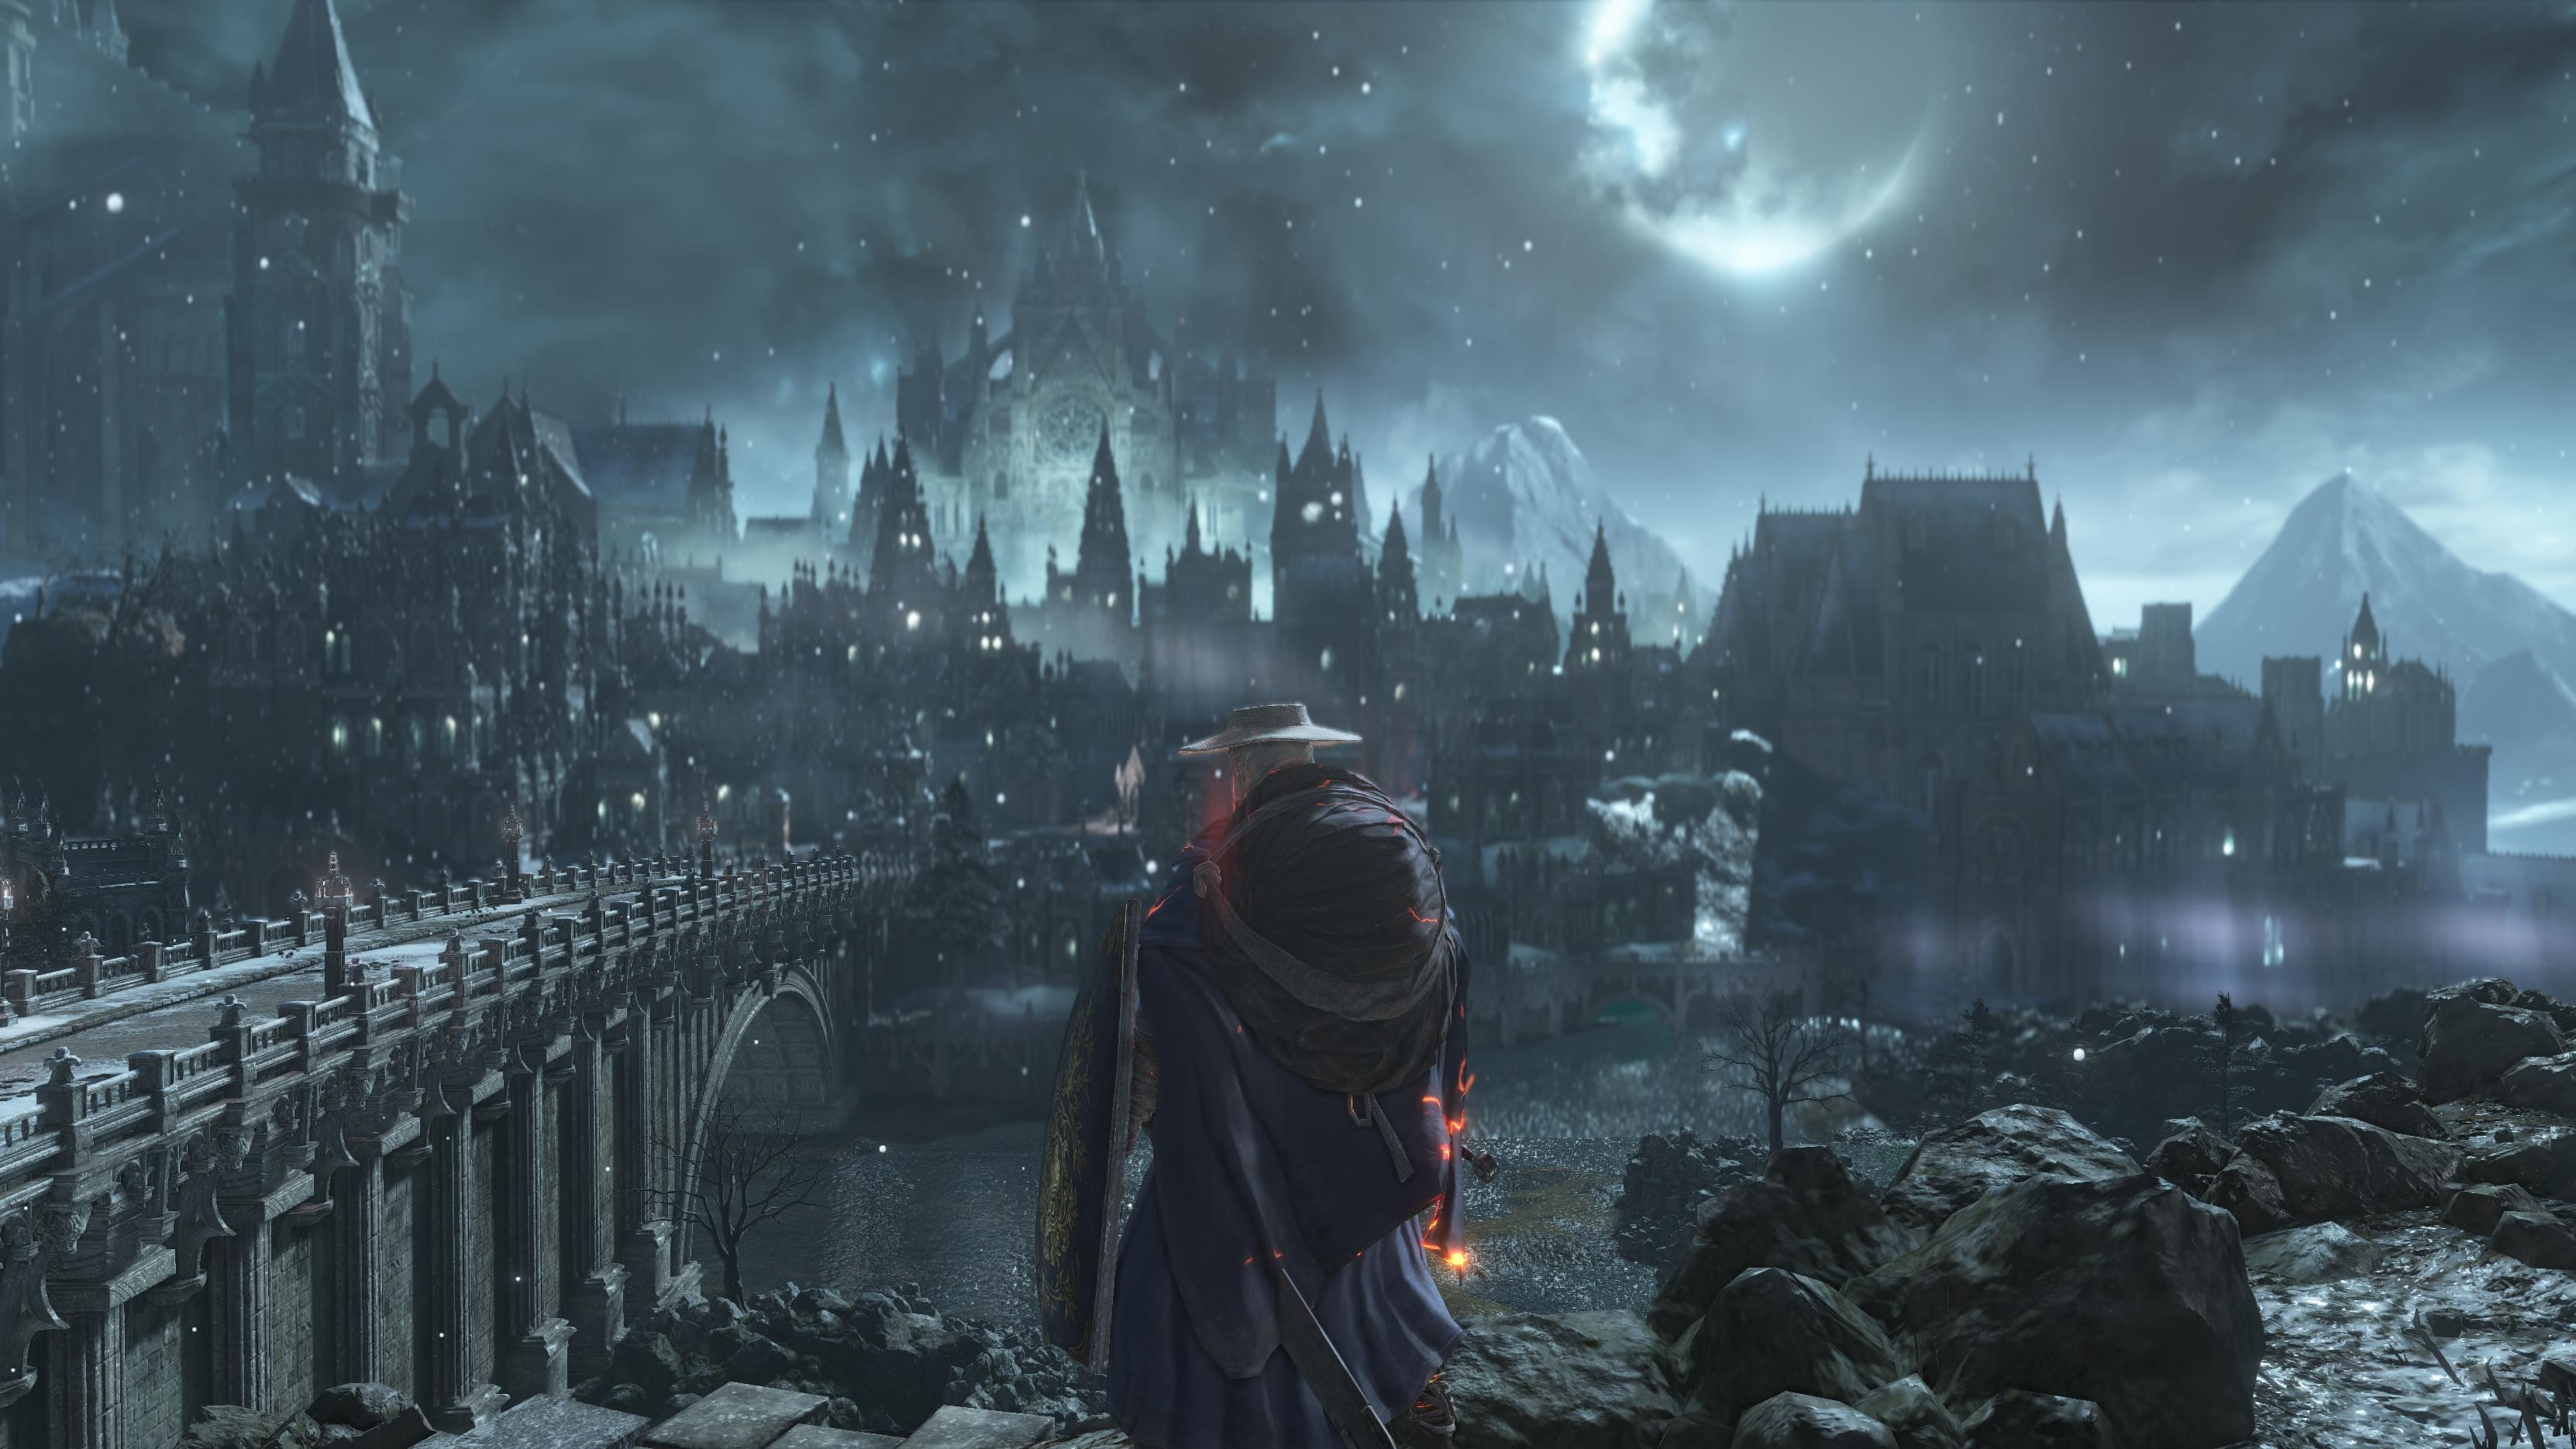
\includegraphics[scale=0.08,keepaspectratio=true]{img/ima1.jpg}
 % colorgama.png: 455x463 px, 96dpi, 12.04x12.25 cm, bb=0 0 341 347
\end{center}
	\begin{itemize}
	\item Limite: "La dimension de la pantalla"
	\item Es importante  atraer al expectador a una escena contreta.
	\end{itemize}
\end{frame}


\subsection{Perspectiva y color}
\begin{frame}

\frametitle{Diseño de Escenario}
\framesubtitle{Perspectiva y color}
\begin{center}


 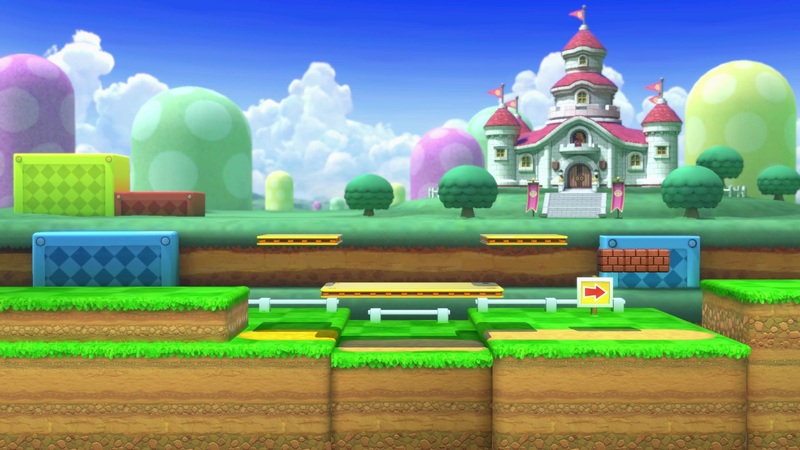
\includegraphics[scale=0.4,keepaspectratio=true]{img/ima2.png}
 % colorgama.png: 455x463 px, 96dpi, 12.04x12.25 cm, bb=0 0 341 347
\end{center}
	\begin{itemize}
	\item La busqueda de generar una ilusion de espacio es importante.
	\item La transmision de sensaciones, el objetivo del videojuego.
	\end{itemize}
\end{frame}

\end{document}

\end{document}
